\chapter{Collection of Results} \label{chp:totalresults}
This appendix is meant as a more or less complete collection of the results obtained in this thesis, with purpose of presenting a complementary picture of the observations. This also allows us to include the (subjective) most important results in the chapter on selected results, \ref{chp:results}, and avoid it to be too overwhelming. However, in this appendix the results will simply be listed and not commented and discussed.

First the computational time will be listed, which are just the information plotted in figure \eqref{fig:cpu_time}. Thereafter we list all the obtained energies, included the distribution between interaction and kinetic energy. We also present a complete set of one-body and two-body densities. 

\section{CPU time} \label{sec:cputime}
The CPU-time was calculated for all the systems we have been looking at, i.e., two-dimensional quantum dots containing up to 90 electrons and three-dimensional quantum dots containing up to 70 particles. Only closed-shell dots were considered, and the times are obviously independent of the frequency. To find correct CPU times per iteration, all systems were run with $M=2^{20}=1,048,576$ cycles per iteration on the computer cluster Abel, every time on 8 nodes á 16 cores. We performed at least four independent runs for each system, where the average time over thousands of iterations was calculated automatically by the program. The results can be found in the tables \eqref{tab:cputime2D} and \eqref{tab:cputime3D} for two- and three dimensional quantum dots respectively. 

\begin{table}[H]
	\caption{The CPU time (in seconds) for each iteration when simulating two-dimensional circular quantum dots of 2-90 electrons. The time was clocked for $M=2^{20}=1,048,576$ Monte Carlo cycles, and to get accurate times we took the average over at least four independent runs with thousands of iterations.}
	\label{tab:cputime2D}
	\begin{tabularx}{\textwidth}{lrR{1.1cm}R{1.1cm}R{1.1cm}R{1.1cm}R{1.1cm}R{1.1cm}R{1.1cm}R{1.1cm}R{1.1cm}} \hline\hline
		\makecell{\\ \phantom{=} \\ \phantom{=}} && 2P & 6P & 12P & 20P & 30P & 42P & 56P & 72P & 90P \\ \hline \\
		RBM && 6.05 & 11.25 & 20.53 & 38.99 & 73.72 & 130.49 & 213.47 & 360.22 & 856.84 \\
		RBM+SJ && 7.12 & 14.07 & 28.42 & 63.27 & 122.93 & 199.60 & 349.22 & - & - \\
		RBM+PJ && 7.26 & 13.50 & 27.68 & 57.09 & 119.17 & 212.53 & 382.13 & - & - \\
		VMC && 5.11 & 10.51 & 20.85 & 41.20 & 76.26 & 137.39 & 230.63 & 355.81 & 544.03 \\ \hline \hline
	\end{tabularx}
\end{table}

\begin{table}[H]
	\caption{The CPU time (in seconds) for each iteration when simulating three-dimensional circular quantum dots of 2-70 electrons. The time was clocked for $M=2^{20}=1,048,576$ Monte Carlo cycles, and to get accurate times we took the average over at least four independent runs with thousands of iterations.}
	\label{tab:cputime3D}
	\begin{tabularx}{\textwidth}{lrR{2.1cm}R{2.1cm}R{2.1cm}R{2.1cm}R{2.1cm}} \hline\hline
		\makecell{\\ \phantom{=} \\ \phantom{=}} && 2P & 8P & 20P & 40P & 70P \\ \hline \\
		RBM && 7.69 & 20.92 & 59.67 & 171.84 & 586.39 \\
		RBM+SJ && 8.95 & 26.86 & 94.64 & 270.92 & - \\
		RBM+PJ && 8.87 & 26.36 & 91.40 & 293.25 & - \\
		VMC && 6.70 & 20.99 & 62.54 & 185.65 & 486.02 \\ \hline \hline
	\end{tabularx}
\end{table}

\section{Ground-state energy} \label{sec:energydistribution}
In this section, we present the ground-state energy included the distribution between kinetic energy, external potential energy and interaction energy for quantum dots containing up to 20 particles in two and three dimensions and with frequencies spanning from $\omega=0.01$ to $\omega=10$. These results are interesting for the validation of the virial theorem, described in section \ref{sec:virial}, but they also makes it possible to compare how the energy spread in two  and three dimensions for an equal number of particles.

We have created respective tables for each of our four methods VMC, RBM, RBM+SJ and RBM+PJ in two and three dimensions, resulting in eight tables in total. We first present VMC, RBM, RBM+SJ and RBM+PJ for two dimensions in that order, and then repeat the same order for three dimensions. 

\subsection{Two dimensions}
\begin{table}[H]
	\caption{This table shows how the total energy ($\langle\hat{H}\rangle$) is distributed between kinetic energy ($\langle\hat{T}\rangle$), external potential energy ($\langle\hat{V}_{\text{ext}}\rangle$) and interaction energy ($\langle\hat{V}_{\text{int}}\rangle$) of two-dimensional circular quantum dots for a wide range of frequencies $\omega$. A plain restricted Boltzmann machine wave function is used. The energy is given in units of $\hbar$, and the numbers in parenthesis are the statistical uncertainties in the last digit.}
	\label{tab:splitfrequencyQDRBM}
	\begin{tabularx}{\textwidth}{R{1cm}rrcR{2.3cm}R{2.3cm}R{2.3cm}R{2.3cm}R{1cm}} \hline\hline
		&\makecell{\\ \phantom{$N$} \\ \phantom{=}} & $\omega$ && \multicolumn{1}{c}{$\langle \hat{H}\rangle$} & \multicolumn{1}{c}{$\langle \hat{T}\rangle$} & \multicolumn{1}{c}{$\langle \hat{V}_{\text{ext}} \rangle$} & \multicolumn{1}{c}{$\langle \hat{V}_{\text{int}} \rangle$} & \\ \hline \\
		&2 & 0.01 && 0.078643(5) & 0.009835(3) & 0.031930(8) & 0.03688(1) \\
		&& 0.1 && 0.4743(1) & 0.08102(8) & 0.2082(2) & 0.1851(2) \\
		&& 0.28 && 1.0707(2) & 0.2047(1) & 0.4678(3) & 0.3983(3) \\
		&& 0.5 && 1.7234(2) & 0.3739(2) & 0.7611(3) & 0.5884(3)\\
		&& 1.0 && 3.0805(2) & 0.7915(2) & 1.3673(4) & 0.9217(3)\\
		&& 2.0 && 5.5936(3) & 1.6377(4) & 2.5507(5) & 1.4051(4) \\
		&& 3.0 && 7.9968(4) & 2.2346(5) & 4.0201(7) & 1.7422(4) \\ 
		&& 5.0 && 12.6070(4) & 3.8768(7) & 6.4292(9) & 2.3010(4) \\
		&& 10.0 && 23.7748(7) & 9.063(3) & 11.132(4) & 3.580(1) \\
		\hdashline \\
		
		&6 & 0.01 && 0.7072(5) & 0.033(2) & 0.2660(4) & 0.4080(6) \\
		&& 0.1 && 3.7337(5) & 0.3251(3) & 1.4070(9) & 2.002(1) \\
		&& 0.28 && 7.9273(9) & 0.8684(6) & 3.009(1) & 4.050(2) \\
		&& 0.5 && 12.241(1) & 1.611(1) & 4.709(2) & 5.921(2)\\
		&& 1.0 && 20.716(1) & 3.391(1) & 7.914(3) & 9.411(2)\\
		&& 2.0 && 36.383(5) & 8.311(7) & 13.705(8) & 14.367(6) \\
		&& 3.0 && 49.415(1) & 10.309(3) & 21.456(4) & 17.649(2) \\ 
		&& 5.0 && 76.801(6) & 23.50(1) & 27.33(1) & 25.967(7) \\
		&& 10.0 && 137.338(4) & 45.25(1) & 55.75(1) & 36.336(6) \\
		\hdashline \\
		
		&12 & 0.01 && 2.5106(8) & 0.0682(2) & 0.893(1) & 1.549(1) \\
		&& 0.1 && 12.703(2) & 0.790(2) & 4.681(3) & 7.232(3) \\
		&& 0.28 && 26.564(3) & 2.254(2) & 9.635(3) & 14.675(4) \\
		&& 0.5 && 40.442(3) & 4.116(2) & 14.868(4) & 21.458(4) \\
		&& 1.0 && 67.614(3) & 8.953(3) & 25.207(6) & 33.455(5) \\
		&& 2.0 && 115.214(5) & 20.760(6) & 43.69(1) & 50.764(7) \\
		&& 3.0 && 158.145(6) & 33.020(8) & 59.72(1) & 65.407(9) \\ 
		&& 5.0 && 239.527(8) & 58.22(1) & 93.92(2) & 87.39(1) \\
		&& 10.0 && 435.36(2) & 114.61(2) & 200.13(4) & 120.62(1) \\
		\hdashline \\
		
		&20 & 0.01 && 6.217(2) & 0.1236(4) & 2.244(2) & 3.849(2) \\
		&& 0.1 && 32.308(5) & 1.708(2) & 7.680(4) & 22.919(7) \\
		&& 0.28 && 63.788(4) & 4.443(3) & 22.707(6) & 36.638(7) \\
		&& 0.5 && 96.491(4) & 8.144(3) & 34.953(8) & 53.394(8) \\
		&& 1.0 && 159.645(5) & 17.12(5) & 58.74(5) & 83.397(9) \\
		&& 2.0 && 269.086(8) & 43.262(8) & 95.17(2) & 130.65(1) \\
		&& 3.0 && 362.52(1) & 57.005(9) & 148.08(2) & 157.43(1) \\ 
		&& 5.0 && 551.21(2) & 115.12(2) & 219.12(4) & 216.97(2) \\
		&& 10.0 && 961.03(4) & 260.2(1) & 364.8(1) & 336.06(7) \\
		\hline \hline
	\end{tabularx}
\end{table} 

\begin{table}[H]
	\caption{This table shows how the total energy ($\langle\hat{H}\rangle$) is distributed between kinetic energy ($\langle\hat{T}\rangle$), external potential energy ($\langle\hat{V}_{\text{ext}}\rangle$) and interaction energy ($\langle\hat{V}_{\text{int}}\rangle$) of two-dimensional circular quantum dots for a wide range of frequencies $\omega$. A restricted Boltzmann machine wave function with a simple Jastrow factor is used. The energy is given in units of $\hbar$, and the numbers in parenthesis are the statistical uncertainties in the last digit.}
	\label{tab:splitfrequencyQDRBMSJ}
	\begin{tabularx}{\textwidth}{R{1cm}rrcR{2.3cm}R{2.3cm}R{2.3cm}R{2.3cm}R{1cm}} \hline\hline
		&\makecell{\\ \phantom{$N$} \\ \phantom{=}} & $\omega$ && \multicolumn{1}{c}{$\langle \hat{H}\rangle$} & \multicolumn{1}{c}{$\langle \hat{T}\rangle$} & \multicolumn{1}{c}{$\langle \hat{V}_{\text{ext}} \rangle$} & \multicolumn{1}{c}{$\langle \hat{V}_{\text{int}} \rangle$} & \\ \hline \\
		&2 & 0.01 && 0.074940(4) & 0.007688(2) & 0.029945(7) & 0.037307(8) \\
		&& 0.1 && 0.44858(6) & 0.07539(8) & 0.1990(2) & 0.1742(1) \\
		&& 0.28 && 1.03470(7) & 0.2163(1) & 0.4547(2) & 0.3637(2) \\
		&& 0.5 && 1.67636(8) & 0.3967(2) & 0.7366(3) & 0.5430(2)\\
		&& 1.0 && 3.0213(1) & 0.8120(2) & 1.3623(4) & 0.8469(3)\\
		&& 2.0 && 5.5254(1) & 1.6572(3) & 2.5447(5) & 1.3234(3) \\
		&& 3.0 && 7.9103(2) & 2.5627(7) & 3.664(1) & 1.6840(5) \\ 
		&& 5.0 && 12.5322(2) & 4.369(1) & 5.890(2) & 2.2838(7) \\
		&& 10.0 && 23.6773(3) & 9.062(3) & 11.208(3) & 3.408(1) \\
		\hdashline \\
		
		&6 & 0.01 && 0.7006(3) & 0.0376(2) & 0.2467(4) & 0.4163(4) \\
		&& 0.1 && 3.6458(4) & 0.2376(3) & 1.3652(9) & 2.043(1) \\
		&& 0.28 && 7.7347(4) & 0.7603(4) & 3.000(1) & 3.974(1) \\
		&& 0.5 && 11.9392(5) & 1.4801(5) & 4.678(1) & 5.781(1) \\
		&& 1.0 && 20.3393(8) & 3.308(1) & 7.983(2) & 9.048(2) \\
		&& 2.0 && 35.2446(8) & 7.098(2) & 14.587(3) & 13.560(2) \\
		&& 3.0 && 49.050(1) & 11.164(3) & 20.6469(5) & 17.240(3) \\ 
		&& 5.0 && 75.116(1) & 19.661(5) & 32.283(7) & 23.172(3) \\
		&& 10.0 && 136.331(2) & 41.65(1) & 60.53(1) & 34.152(5) \\
		\hdashline \\
		
		&12 & 0.01 && 2.4950(5) & 0.07(2) & 0.845(4) & 1.58(2) \\
		&& 0.1 && 12.5964(7) & 0.4520(4) & 4.644(1) & 7.500(1) \\
		&& 0.28 && 26.071(1) & 1.7279(8) & 9.672(3) & 14.670(3) \\
		&& 0.5 && 39.6340(7) & 3.4852(5) & 14.948(2) & 21.201(2) \\
		&& 1.0 && 66.1898(8) & 7.8777(8) & 25.822(2) & 32.490(2) \\
		&& 2.0 && 112.502(2) & 18.118(4) & 44.118(4) & 50.201(6) \\
		&& 3.0 && 154.521(3) & 28.050(5) & 63.84(1) & 62.634(6) \\ 
		&& 5.0 && 234.110(6) & 52.86(1) & 94.50(2) & 86.75(1) \\
		&& 10.0 && 415.384(7) & 108.57(2) & 181.90(3) & 124.92(1) \\
		\hdashline \\
		
		&20 & 0.01 && 6.239(2) & 0.1372(6) & 2.184(2) & 3.919(3) \\
		&& 0.1 && 30.624(3) & 1.487(2) & 10.893(5) & 18.243(5) \\
		&& 0.28 && 62.786(3) & 3.190(2) & 22.782(7) & 36.814(6) \\
		&& 0.5 && 94.755(3) & 6.709(2) & 34.845(7) & 53.200(6) \\
		&& 1.0 && 156.816(4) & 15.340(3) & 59.931(9) & 81.545(7) \\
		&& 2.0 && 265.66(9) & 39.31(8) & 95.78(1) & 130.57(2) \\
		&& 3.0 && 360.630(6) & 58.36(1) & 141.54(2) & 160.72(2) \\ 
		&& 5.0 && 543.06(1) & 112.38(2) & 210.52(4) & 220.15(2) \\
		&& 10.0 && 952.71(2) & 237.65(4) & 392.06(7) & 323.00(3) \\
		\hline\hline
	\end{tabularx}
\end{table}

\begin{table}[H]
	\caption{This table shows how the total energy ($\langle\hat{H}\rangle$) is distributed between kinetic energy ($\langle\hat{T}\rangle$), external potential energy ($\langle\hat{V}_{\text{ext}}\rangle$) and interaction energy ($\langle\hat{V}_{\text{int}}\rangle$) of two-dimensional circular quantum dots for a wide range of frequencies $\omega$. A restricted Boltzmann machine with Padé-Jastrow wave function is used. The energy is given in units of $\hbar$, and the numbers in parenthesis are the statistical uncertainties in the last digit.}
	\label{tab:splitfrequencyQDRBMPJ}
	\begin{tabularx}{\textwidth}{R{1cm}rrcR{2.3cm}R{2.3cm}R{2.3cm}R{2.3cm}R{1cm}} \hline\hline
		&\makecell{\\ \phantom{$N$} \\ \phantom{=}} & $\omega$ && \multicolumn{1}{c}{$\langle \hat{H}\rangle$} & \multicolumn{1}{c}{$\langle \hat{T}\rangle$} & \multicolumn{1}{c}{$\langle \hat{V}_{\text{ext}} \rangle$} & \multicolumn{1}{c}{$\langle \hat{V}_{\text{int}} \rangle$} & \\ \hline \\
		&2 & 0.01 && 0.074107(8) & 0.01031(3) & 0.02703(4) & 0.03677(3) \\
		&& 0.1 && 0.440975(8) & 0.09223(9) & 0.1757(1) & 0.17304(9) \\
		&& 0.28 && 1.021668(7) & 0.2468(1) & 0.4258(2) & 0.3490(1) \\
		&& 0.5 && 1.659637(6) & 0.4305(2) & 0.7112(2) & 0.5179(2) \\
		&& 1.0 && 2.999587(5) & 0.8440(3) & 1.3418(3) & 0.8238(2) \\
		&& 2.0 && 5.49475(1) & 1.7234(4) & 2.4657(4) & 1.3057(3) \\
		&& 3.0 && 7.87961(1) & 2.3144(5) & 3.9349(6) & 1.6413(3) \\
		&& 5.0 && 12.49832(1) & 3.9569(7) & 6.3068(8) & 2.2347(4) \\
		&& 10.0 && 23.65275(7) & 9.228(3) & 11.059(3) & 3.366(1) \\
		\hdashline \\
		
		&6 & 0.01 && 0.6932(5) & 0.031(2) & 0.260(2) & 0.401(1) \\
		&& 0.1 && 3.5700(2) & 0.3494(3) & 1.2805(9) & 1.9401(8) \\
		&& 0.28 && 7.6203(2) & 0.9519(6) & 2.82(1) & 3.84(1) \\
		&& 0.5 && 11.8074(2) & 1.7018(7) & 4.513(1) & 5.5927(9) \\
		&& 1.0 && 20.1832(1) & 3.428(1) & 8.068(1) & 8.687(1) \\
		&& 2.0 && 35.0872(3) & 7.670(2) & 14.139(3) & 13.279(2) \\
		&& 3.0 && 48.9157(8) & 10.789(5) & 20.383(5) & 17.743(2) \\ 
		&& 5.0 && 74.9545(5) & 20.402(5) & 31.744(7) & 22.809(3) \\
		&& 10.0 && 136.1738(8) & 42.66(1) & 59.71(1) & 33.799(5) \\
		\hdashline \\
		
		&12 & 0.01 && 2.5019(4) & 0.0699(2) & 0.893(1) & 1.539(1) \\
		&& 0.1 && 12.361(1) & 0.797(1) & 4.394(3) & 7.169(3) \\
		&& 0.28 && 25.7461(6) & 2.415(1) & 9.050(2) & 14.281(2) \\
		&& 0.5 && 39.2661(6) & 4.262(2) & 14.277(2) & 20.728(2) \\
		&& 1.0 && 65.7911(5) & 8.537(3) & 25.197(4) & 32.067(3) \\
		&& 2.0 && 111.9426(5) & 17.817(3) & 46.532(4) & 47.593(3) \\
		&& 3.0 && 154.206(1) & 29.701(6) & 60.74(1) & 63.763(7) \\ 
		&& 5.0 && 233.633(4) & 58.33(1) & 84.76(1) & 90.537(9) \\
		&& 10.0 && 415.943(9) & 124.13(2) & 157.92(3) & 133.89(1) \\
		\hdashline \\
		
		&20 & 0.01 && 6.210(1) & 0.1208(5) & 2.189(2) & 3.900(2) \\
		&& 0.1 && 30.156(1) & 1.574(1) & 10.473(3) & 18.109(3) \\
		&& 0.28 && 62.210(1) & 4.657(2) & 21.227(4) & 36.106(4) \\
		&& 0.5 && 94.127(1) & 8.249(3) & 33.543(5) & 52.335(4) \\
		&& 1.0 && 156.099(1) & 16.768(6) & 58.513(8) & 80.818(6) \\
		&& 2.0 && 262.598(1) & 34.758(6) & 108.546(9) & 119.293(7) \\
		&& 3.0 && 359.072(4) & 60.75(2) & 140.51(4) & 157.82(2) \\ 
		&& 5.0 && 539.13(1) & 120.09(2) & 188.45(2) & 230.58(1) \\
		&& 10.0 && 947.33(2) & 257.67(5) & 348.35(6) & 341.31(3) \\
		\hline \hline
	\end{tabularx}
\end{table} 
\begin{table}[H]
	\caption{This table shows how the total energy ($\langle\hat{H}\rangle$) is distributed between kinetic energy ($\langle\hat{T}\rangle$), external potential energy ($\langle\hat{V}_{\text{ext}}\rangle$) and interaction energy ($\langle\hat{V}_{\text{int}}\rangle$) of two-dimensional circular quantum dots for a wide range of frequencies $\omega$. A standard variational Monte-Carlo wave function is used. The energy is given in units of $\hbar$, and the numbers in parenthesis are the statistical uncertainties in the last digit.}
	\label{tab:splitfrequencyQDVMC}
	\begin{tabularx}{\textwidth}{R{1cm}rrcR{2.3cm}R{2.3cm}R{2.3cm}R{2.3cm}R{1cm}} \hline\hline
		&\makecell{\\ \phantom{$N$} \\ \phantom{=}} & $\omega$ && \multicolumn{1}{c}{$\langle \hat{H}\rangle$} & \multicolumn{1}{c}{$\langle \hat{T}\rangle$} & \multicolumn{1}{c}{$\langle \hat{V}_{\text{ext}} \rangle$} & \multicolumn{1}{c}{$\langle \hat{V}_{\text{int}} \rangle$} & \\ \hline \\
		&2 & 0.01 && 0.074070(8) & 0.00947(3) & 0.02732(5) & 0.03728(4) \\
		&& 0.1 && 0.44129(1) & 0.09117(9) & 0.1789(1) & 0.17119(9) \\
		&& 0.28 && 1.02192(1) & 0.2477(1) & 0.4256(2) & 0.3487(1) \\
		&& 0.5 && 1.65974(1) & 0.4346(2) & 0.7057(2) & 0.5195(2)\\
		&& 1.0 && 2.99936(1) & 0.8523(3) & 1.3149(3) & 0.8321(2)\\
		&& 2.0 && 5.49689(4) & 1.811(2) & 2.403(2) & 1.283(1) \\
		&& 3.0 && 7.88401(4) & 2.732(2) & 3.500(3) & 1.652(1) \\ 
		&& 5.0 && 12.50405(5) & 4.619(4) & 5.629(4) & 2.255(2) \\
		&& 10.0 && 23.65035(1) & 9.529(1) & 10.538(1) & 3.583(1) \\
		\hdashline \\
		
		&6 & 0.01 && 0.6982(1) & 0.02735(7) & 0.2427(3) & 0.4281(3) \\
		&& 0.1 && 3.5695(1) & 0.3201(3) & 1.2934(6) & 1.9560(5) \\
		&& 0.28 && 7.6219(1) & 0.9105(4) & 2.8821(9) & 3.8292(7) \\
		&& 0.5 && 11.8104(2) & 1.6710(7) & 4.535(1) & 5.6045(9) \\
		&& 1.0 && 20.1918(2) & 3.405(1) & 8.046(1) & 8.741(1) \\
		&& 2.0 && 35.0734(3) & 7.751(2) & 13.846(3) & 13.476(2) \\
		&& 3.0 && 48.8728(4) & 12.016(2) & 19.682(4) & 17.175(2) \\ 
		&& 5.0 && 74.9356(5) & 20.796(4) & 31.043(6) & 23.097(3) \\
		&& 10.0 && 136.1522(7) & 43.712(9) & 58.20(1) & 34.240(5) \\
		\hdashline \\
		
		&12 & 0.01 && 2.4972(3) & 0.05506(2) & 0.858(1) & 1.584(1)\\
		&& 0.1 && 12.3196(3) & 0.6885(6) & 4.393(2) & 7.238(2) \\
		&& 0.28 && 25.7049(4) & 2.090(1) & 9.355(2) & 14.260(2) \\
		&& 0.5 && 39.2421(5) & 3.939(2) & 14.564(3) & 20.739(3) \\
		&& 1.0 && 65.7026(4) & 9.246(2) & 23.079(3) & 33.378(3) \\
		&& 2.0 && 111.8377(3) & 19.678(2) & 41.349(3) & 50.811(2) \\
		&& 3.0 && 154.206(1) & 29.701(6) & 60.74(1) & 63.763(7) \\ 
		&& 5.0 && 232.818(2) & 56.157(9) & 88.18(1) & 88.478(9) \\
		&& 10.0 && 415.056(4) & 112.99(2) & 173.91(3) & 128.15(1) \\
		\hdashline \\
		
		&20 & 0.01 && 6.2097(8) & 0.1005(4) & 2.270(3) & 3.839(3) \\
		&& 0.1 && 30.086(1) & 1.243(1) & 10.587(4) & 18.257(4) \\
		&& 0.28 && 62.0755(7) & 3.902(2) & 22.228(5) & 35.946(4) \\
		&& 0.5 && 94.0433(9) & 7.823(3) & 33.938(6) & 52.282(5) \\
		&& 1.0 && 155.8900(4) & 17.921(2) & 54.076(3) & 83.893(3) \\
		&& 2.0 && 262.5339(9) & 38.402(3) & 95.681(7) & 128.451(5) \\
		&& 3.0 && 358.927(1) & 61.017(5) & 133.99(1) & 163.924(7) \\ 
		&& 5.0 && 542.680(7) & 127.77(2) & 177.89(2) & 237.12(2) \\
		&& 10.0 && 945.596(8) & 231.56(4) & 389.26(7) & 324.77(3) \\
		\hline \hline
	\end{tabularx}
\end{table} 

\subsection{Three dimensions}
\begin{table}[H]
	\caption{This table shows how the total energy ($\langle\hat{H}\rangle$) is distributed between kinetic energy ($\langle\hat{T}\rangle$), external potential energy ($\langle\hat{V}_{\text{ext}}\rangle$) and interaction energy ($\langle\hat{V}_{\text{int}}\rangle$) of three-dimensional circular quantum dots for a wide range of frequencies $\omega$. A plain restricted Boltzmann machine wave function is used. The energy is given in units of $\hbar$, and the numbers in parenthesis are the statistical uncertainties in the last digit.}
	\label{tab:splitfrequencyQDRBM3D}
	\begin{tabularx}{\textwidth}{R{1cm}rrcR{2.3cm}R{2.3cm}R{2.3cm}R{2.3cm}R{1cm}} \hline\hline
		&\makecell{\\ \phantom{$N$} \\ \phantom{=}} & $\omega$ && \multicolumn{1}{c}{$\langle \hat{H}\rangle$} & \multicolumn{1}{c}{$\langle \hat{T}\rangle$} & \multicolumn{1}{c}{$\langle \hat{V}_{\text{ext}} \rangle$} & \multicolumn{1}{c}{$\langle \hat{V}_{\text{int}} \rangle$} & \\ \hline \\
		&2 & 0.01 && 0.85193(5) & 0.014853(4) & 0.03141(9) & 0.03893(1) \\
		&& 0.1 && 0.5177(1) & 0.1249(1) & 0.2065(2) & 0.1863(2) \\
		&& 0.28 && 1.2261(1) & 0.35(2) & 0.53(2) & 0.3488(6) \\
		&& 0.5 && 2.0269(1) & 0.6595(3) & 0.8778(4) & 0.4896(2) \\
		&& 1.0 && 3.7574(1) & 1.3224(5) & 1.7215(5) & 0.7136(2) \\
		&& 2.0 && 7.0870(1) & 2.7338(6) & 3.3183(7) & 1.0350(2) \\
		&& 3.0 && 10.2981(2) & 3.7507(8) & 5.2896(9) & 1.2578(2) \\ 
		&& 5.0 && 16.7018(1) & 6.211(1) & 8.890(1) & 1.6012(2) \\
		&& 10.0 && 32.2186(2) & 7.879(3) & 22.306(3) & 2.0343(2) \\
		\hdashline \\
		
		&8 & 0.01 && 1.1350(1) & 0.0626(2) & 0.3951(7) & 0.6774(7) \\
		&& 0.1 && 5.8910(6) & 0.6480(6) & 2.075(2) & 3.168(2) \\
		&& 0.28 && 12.650(1) & 1.931(1) & 4.641(2) & 6.078(2) \\
		&& 0.5 && 19.680(2) & 3.601(2) & 7.289(4) & 8.786(3) \\
		&& 1.0 && 33.305(1) & 7.032(2) & 12.267(3) & 14.006(2) \\
		&& 2.0 && 58.889(3) & 16.976(4) & 19.717(5) & 22.195(3) \\
		&& 3.0 && 81.648(3) & 23.987(6) & 31.157(8) & 26.504(4) \\ 
		&& 5.0 && 126.03(9) & 42.68(6) & 47.58(5) & 35.77(2) \\
		&& 10.0 && 231.410(6) & 85.62(2) & 95.00(2) & 50.789(7) \\
		\hdashline \\
		
		&20 & 0.01 && 5.6448(4) & 0.1624(4) & 1.955(2) & 3.527(2) \\
		&& 0.1 && 27.9277(5) & 1.7925(5) & 9.676(2) & 16.459(2) \\
		&& 0.28 && 57.822(1) & 5.240(1) & 20.384(4) & 32.198(3) \\
		&& 0.5 && 87.798(5) & 9.635(5) & 32.12(1) & 46.047(9) \\
		&& 1.0 && 147.407(3) & 22.085(5) & 52.32(1) & 73.003(8) \\
		&& 2.0 && 250.159(7) & 49.76(1) & 83.69(2) & 116.71(1) \\
		&& 3.0 && 335.440(5) & 64.59(1) & 130.27(2) & 140.578(9) \\ 
		&& 5.0 && 524.94(2) & 121.39(3) & 225.61(5) & 177.94(2) \\
		&& 10.0 && 1005.24(6) & 225.76(5) & 552.3(1) & 227.20(2) \\
		\hline \hline
	\end{tabularx}
\end{table}

\begin{table}[H]
	\caption{This table shows how the total energy ($\langle\hat{H}\rangle$) is distributed between kinetic energy ($\langle\hat{T}\rangle$), external potential energy ($\langle\hat{V}_{\text{ext}}\rangle$) and interaction energy ($\langle\hat{V}_{\text{int}}\rangle$) of three-dimensional circular quantum dots for a wide range of frequencies $\omega$. A restricted Boltzmann machine with a simple Jastrow factor is used. The energy is given in units of $\hbar$, and the numbers in parenthesis are the statistical uncertainties in the last digit.}
	\label{tab:splitfrequencyQDRBMSJ3D}
	\begin{tabularx}{\textwidth}{R{1cm}rrcR{2.3cm}R{2.3cm}R{2.3cm}R{2.3cm}R{1cm}} \hline\hline
		&\makecell{\\ \phantom{$N$} \\ \phantom{=}} & $\omega$ && \multicolumn{1}{c}{$\langle \hat{H}\rangle$} & \multicolumn{1}{c}{$\langle \hat{T}\rangle$} & \multicolumn{1}{c}{$\langle \hat{V}_{\text{ext}} \rangle$} & \multicolumn{1}{c}{$\langle \hat{V}_{\text{int}} \rangle$} \\ \hline \\
		&2 & 0.01 && 0.07994(2) & 0.01069(3) & 0.03190(8) & 0.03735(8) \\
		&& 0.1 && 0.50214(3) & 0.1178(1) & 0.2177(2) & 0.1666(1) \\
		&& 0.28 && 1.20475(4) & 0.3497(2) & 0.5326(3) & 0.3225(1) \\
		&& 0.5 && 2.00371(4) & 0.6340(3) & 0.9201(4) & 0.4496(2) \\
		&& 1.0 && 3.73543(4) & 1.2801(4) & 1.7871(5) & 0.6683(2) \\
		&& 2.0 && 7.06343(7) & 2.7117(7) & 3.3574(9) & 0.9944(2) \\
		&& 3.0 && 10.32289(5) & 3.5281(8) & 5.6147(9) & 1.1801(2) \\ 
		&& 5.0 && 16.7155(1) & 7.035(2) & 8.035(2) & 1.6462(4) \\
		&& 10.0 && 32.6045(9) & 14.568(4) & 15.613(5) & 2.4238(6) \\
		\hdashline \\
		
		&8 & 0.01 && 1.1371(5) & 0.02(1) & 0.388(6) & 0.73(2) \\
		&& 0.1 && 5.7498(4) & 0.4107(3) & 2.113(1) & 3.226(1) \\
		&& 0.28 && 12.2492(4) & 1.3909(6) & 4.756(2) & 6.101(1) \\
		&& 0.5 && 19.0241(4) & 2.7417(9) & 7.579(2) & 8.704(2) \\
		&& 1.0 && 32.7159(6) & 6.137(1) & 13.440(3) & 13.139(2) \\
		&& 2.0 && 57.4473(8) & 13.451(3) & 24.361(5) & 19.636(2) \\
		&& 3.0 && 80.6370(9) & 21.039(5) & 34.888(8) & 24.710(3) \\ 
		&& 5.0 && 124.955(1) & 37.126(9) & 54.81(1) & 33.020(5) \\
		&& 10.0 && 230.149(2) & 76.75(2) & 105.83(2) & 47.560(6) \\
		\hdashline \\
		
		&20 & 0.01 && 5.6448(4) & 0.1624(4) & 1.955(2) & 3.527(2) \\
		&& 0.1 && 27.470(1) & 0.9593(9) & 9.711(6) & 16.800(5) \\
		&& 0.28 && 56.600(1) & 3.515(1) & 20.616(7) & 32.469(6) \\
		&& 0.5 && 85.893(1) & 7.212(2) & 31.722(8) & 46.958(7) \\
		&& 1.0 && 143.209(2) & 16.531(7) & 54.86(1) & 71.819(7) \\
		&& 2.0 && 242.195(2) & 37.591(8) & 96.36(2) & 108.24(1) \\
		&& 3.0 && 333.07(6) & 53.2(5) & 138.0(5) & 141.835(9) \\ 
		&& 5.0 && 507.35(1) & 119.91(2) & 196.89(4) & 190.55(2) \\
		&& 10.0 && 903.79(2) & 253.59(5) & 372.83(7) & 277.37(3) \\
		\hline \hline
	\end{tabularx}
\end{table}

\begin{table}[H]
	\caption{This table shows how the total energy ($\langle\hat{H}\rangle$) is distributed between kinetic energy ($\langle\hat{T}\rangle$), external potential energy ($\langle\hat{V}_{\text{ext}}\rangle$) and interaction energy ($\langle\hat{V}_{\text{int}}\rangle$) of three-dimensional circular quantum dots for a wide range of frequencies $\omega$. A restricted Boltzmann machine with Padé-Jastrow wave function is used. The energy is given in units of $\hbar$, and the numbers in parenthesis are the statistical uncertainties in the last digit.}
	\label{tab:splitfrequencyQDRBMPJ3D}
	\begin{tabularx}{\textwidth}{R{1cm}rrcR{2.3cm}R{2.3cm}R{2.3cm}R{2.3cm}R{1cm}} \hline\hline
		&\makecell{\\ \phantom{$N$} \\ \phantom{=}} & $\omega$ && \multicolumn{1}{c}{$\langle \hat{H}\rangle$} & \multicolumn{1}{c}{$\langle \hat{T}\rangle$} & \multicolumn{1}{c}{$\langle \hat{V}_{\text{ext}} \rangle$} & \multicolumn{1}{c}{$\langle \hat{V}_{\text{int}} \rangle$} & \\ \hline \\
		&2 & 0.01 && 0.079312(6) & 0.01283(4) & 0.02987(6) & 0.03661(4) \\
		&& 0.1 && 0.500080(6) & 0.1271(1) & 0.2085(2) & 0.1644(1) \\
		&& 0.28 && 1.201710(6) & 0.3624(2) & 0.5253(3) & 0.3140(1) \\
		&& 0.5 && 1.999912(5) & 0.6515(3) & 0.9040(3) & 0.4444(1) \\
		&& 1.0 && 3.729827(5) & 1.2995(4) & 1.7688(5) & 0.6615(2) \\
		&& 2.0 && 7.05785(1) & 2.7017(6) & 3.3705(6) & 0.9856(1) \\
		&& 3.0 && 10.31271(4) & 3.5410(8) & 5.5989(9) & 1.1728(2) \\ 
		&& 5.0 && 16.7170(1) & 7.012(2) & 8.072(2) & 1.632(4) \\
		&& 10.0 && 32.44255(9) & 8.054(3) & 22.384(3) & 2.0042(2) \\
		\hdashline \\
		
		&8 & 0.01 && 1.1346(1) & 0.0624(2) & 0.3910(7) & 0.6812(7) \\
		&& 0.1 && 5.8562(9) & 0.6134(7) & 2.088(2) & 3.155(2) \\
		&& 0.28 && 12.2056(2) & 1.5665(7) & 4.605(1) & 6.034(1) \\
		&& 0.5 && 18.9747(2) & 2.972(1) & 7.344(2) & 8.659(1) \\
		&& 1.0 && 32.6820(2) & 6.266(2) & 13.390(3) & 13.026(1) \\
		&& 2.0 && 57.4148(3) & 13.744(3) & 24.205(5) & 19.466(2) \\
		&& 3.0 && 80.6280(3) & 18.35(2) & 38.64(2) & 23.627(2) \\ 
		&& 5.0 && 124.915(1) & 37.61(2) & 54.44(2) & 32.87(8) \\
		&& 10.0 && 230.186(1) & 78.64(4) & 103.59(5) & 47.95(1) \\
		\hdashline \\
		
		&20 & 0.01 && 5.6328(3) & 0.1621(4) & 1.923(2) & 3.558(2) \\
		&& 0.1 && 27.3382(8) & 1.336(3) & 9.408(4) & 16.595(3) \\
		&& 0.28 && 56.4477(6) & 4.157(2) & 20.124(4) & 32.167(4) \\
		&& 0.5 && 85.7153(6) & 8.028(2) & 31.333(6) & 46.354(4) \\
		&& 1.0 && 142.9409(6) & 17.603(3) & 54.592(7) & 70.746(5) \\
		&& 2.0 && 242.1168(8) & 38.487(5) & 96.23(1) & 107.403(7) \\
		&& 3.0 && 333.027(1) & 49.3(3) & 152.1(3) & 131.618(7) \\ 
		&& 5.0 && 506.58(1) & 130.79(3) & 172.35(3) & 203.45(2) \\
		&& 10.0 && 897.68(2) & 273.53(5) & 328.64(6) & 295.52(3) \\
		\hline \hline
	\end{tabularx}
\end{table}
\begin{table}[H]
	\caption{This table shows how the total energy ($\langle\hat{H}\rangle$) is distributed between kinetic energy ($\langle\hat{T}\rangle$), external potential energy ($\langle\hat{V}_{\text{ext}}\rangle$) and interaction energy ($\langle\hat{V}_{\text{int}}\rangle$) of three-dimensional circular quantum dots for a wide range of frequencies $\omega$. A standard variational Monte-Carlo wave function is used. The energy is given in units of $\hbar$, and the numbers in parenthesis are the statistical uncertainties in the last digit.}
	\label{tab:splitfrequencyQDVMC3D}
	\begin{tabularx}{\textwidth}{R{1cm}rrcR{2.3cm}R{2.3cm}R{2.3cm}R{2.3cm}R{1cm}} \hline\hline
		&\makecell{\\ \phantom{$N$} \\ \phantom{=}} & $\omega$ && \multicolumn{1}{c}{$\langle \hat{H}\rangle$} & \multicolumn{1}{c}{$\langle \hat{T}\rangle$} & \multicolumn{1}{c}{$\langle \hat{V}_{\text{ext}} \rangle$} & \multicolumn{1}{c}{$\langle \hat{V}_{\text{int}} \rangle$} & \\ \hline \\
		&2 & 0.01 && 0.079284(6) & 0.01221(4) & 0.039757(6) & 0.036319(4) \\
		&& 0.1 && 0.500083(7) & 0.1263(1) & 0.2082(2) & 0.1656(1) \\
		&& 0.28 && 1.201752(6) & 0.3606(2) & 0.5272(3) & 0.3140(1) \\
		&& 0.5 && 1.999977(5) & 0.6517(3) & 0.9032(3) & 0.4451(1) \\
		&& 1.0 && 3.730030(5) & 1.3105(4) & 1.7551(5) & 0.6644(2) \\
		&& 2.0 && 7.065911(7) & 3.2766(4) & 2.6932(5) & 1.0961(2) \\
		&& 3.0 && 10.31717(1) & 3.8365(7) & 5.2770(8) & 1.2037(2) \\ 
		&& 5.0 && 16.713925(4) & 8.1523(8) & 6.7797(9) & 1.7819(2) \\
		&& 10.0 && 32.449053(8) & 14.586(2) & 15.470(2) & 2.3933(2) \\
		\hdashline \\
		
		&8 & 0.01 && 1.12283(7) & 0.04384(7) & 0.3832(2) & 0.6958(2) \\
		&& 0.1 && 5.7126(1) & 0.4930(4) & 2.085(1) & 3.1342(9) \\
		&& 0.28 && 12.2050(2) & 1.5332(7) & 4.630(2) & 6.041(1) \\
		&& 0.5 && 18.96747(8) & 3.2098(4) & 6.7892(8) & 8.9647(6) \\
		&& 1.0 && 32.6863(2) & 6.244(2) & 13.378(3) & 13.064(1) \\
		&& 2.0 && 57.4197(5) & 14.344(6) & 23.14(1) & 19.932(5) \\
		&& 3.0 && 80.6193(3) & 22.281(5) & 33.286(7) & 25.052(3) \\ 
		&& 5.0 && 124.9024(4) & 38.713(8) & 52.89(1) & 33.300(4) \\
		&& 10.0 && 230.1668(7) & 81.03(2) & 100.56(2) & 48.573(6) \\
		\hdashline \\
		
		&20 & 0.01 && 5.6428(3) & 0.1621(4) & 1.923(2) & 3.558(2) \\
		&& 0.1 && 27.3152(5) & 1.247(1) & 9.392(3) & 16.676(3) \\
		&& 0.28 && 56.4386(5) & 3.991(2) & 20.125(5) & 32.322(4) \\
		&& 0.5 && 85.7197(6) & 7.868(2) & 31.383(6) & 46.469(5) \\
		&& 1.0 && 142.9561(7) & 17.29(2) & 54.45(3) & 71.218(6) \\
		&& 2.0 && 242.0320(6) & 42.246(3) & 86.317(9) & 113.469(6) \\
		&& 3.0 && 332.6976(6) & 67.976(5) & 119.95(1) & 144.772(7) \\ 
		&& 5.0 && 509.45(1) & 137.93(2) & 163.28(3) & 208.24(2) \\
		&& 10.0 && 902.58(2) & 288.99(4) & 310.87(5) & 302.72(3) \\
		\hline \hline
	\end{tabularx}
\end{table}

\begin{landscape}
	\section{One-body density plots} \label{sec:onebody}
	\begin{figure}[H]
		\centering
		\captionsetup[subfigure]{labelformat=empty}
		\captionsetup{width=0.9\hsize}
		\subfloat{\raisebox{2cm}{\rotatebox[origin=t]{90}{2P}}}\hspace{0.1cm}
		\subfloat{{\includegraphics[width=5.7cm]{/home/evenmn/VMC/plots/int1/onebody/2D/2P/0.100000w/ADAM_MC1048576.png}}}
		\subfloat{{\includegraphics[width=5.7cm]{/home/evenmn/VMC/plots/int1/onebody/2D/2P/0.280000w/ADAM_MC1048576.png}}}
		\subfloat{{\includegraphics[width=5.7cm]{/home/evenmn/VMC/plots/int1/onebody/2D/2P/0.500000w/ADAM_MC1048576.png}}}
		\subfloat{{\includegraphics[width=5.7cm]{/home/evenmn/VMC/plots/int1/onebody/2D/2P/1.000000w/ADAM_MC1048576.png}}}\\ [-0.5cm]
		
		\subfloat{\raisebox{2cm}{\rotatebox[origin=t]{90}{6P}}}\hspace{0.1cm}
		\subfloat{{\includegraphics[width=5.7cm]{/home/evenmn/VMC/plots/int1/onebody/2D/6P/0.100000w/ADAM_MC1048576.png}}}
		\subfloat{{\includegraphics[width=5.7cm]{/home/evenmn/VMC/plots/int1/onebody/2D/6P/0.280000w/ADAM_MC1048576.png}}}
		\subfloat{{\includegraphics[width=5.7cm]{/home/evenmn/VMC/plots/int1/onebody/2D/6P/0.500000w/ADAM_MC1048576.png}}}
		\subfloat{{\includegraphics[width=5.7cm]{/home/evenmn/VMC/plots/int1/onebody/2D/6P/1.000000w/ADAM_MC1048576.png}}}\\ [-0.5cm]
		
		\subfloat{\raisebox{2cm}{\rotatebox[origin=t]{90}{12P}}}\hspace{0.1cm}
		\subfloat[$\omega=0.1$]{{\includegraphics[width=5.7cm]{/home/evenmn/VMC/plots/int1/onebody/2D/12P/0.100000w/ADAM_MC1048576.png}}}
		\subfloat[$\omega=0.28$]{{\includegraphics[width=5.7cm]{/home/evenmn/VMC/plots/int1/onebody/2D/12P/0.280000w/ADAM_MC1048576.png}}}
		\subfloat[$\omega=0.5$]{{\includegraphics[width=5.7cm]{/home/evenmn/VMC/plots/int1/onebody/2D/12P/0.500000w/ADAM_MC1048576.png}}}
		\subfloat[$\omega=1.0$]{{\includegraphics[width=5.7cm]{/home/evenmn/VMC/plots/int1/onebody/2D/12P/1.000000w/ADAM_MC1048576.png}}}
		
		%\caption{Radial one-body density plots for two-dimensional circular quantum dots with 2, 6 and 12 interacting electrons for the oscillator frequencies $\omega=0.1$, 0.28, 0.5, 1.0. ADAM optimizer was used and after convergence the number of Monte-Carlo cycles was $M=2^{28}=268,435,456$. The methods are detailed in the introductory words to chapter \ref{chp:results}.}
		\label{fig:OB_interaction_2D_1}
	\end{figure}
	\begin{figure}[H]
		\centering
		\captionsetup[subfigure]{labelformat=empty}
		\captionsetup{width=0.9\hsize}
		\subfloat{\raisebox{2cm}{\rotatebox[origin=t]{90}{20P}}}\hspace{0.1cm}
		\subfloat{{\includegraphics[width=5.7cm]{/home/evenmn/VMC/plots/int1/onebody/2D/20P/0.100000w/ADAM_MC1048576.png}}}
		\subfloat{{\includegraphics[width=5.7cm]{/home/evenmn/VMC/plots/int1/onebody/2D/20P/0.280000w/ADAM_MC1048576.png}}}
		\subfloat{{\includegraphics[width=5.7cm]{/home/evenmn/VMC/plots/int1/onebody/2D/20P/0.500000w/ADAM_MC1048576.png}}}
		\subfloat{{\includegraphics[width=5.7cm]{/home/evenmn/VMC/plots/int1/onebody/2D/20P/1.000000w/ADAM_MC1048576.png}}}\\ [-0.5cm]
		
		\subfloat{\raisebox{2cm}{\rotatebox[origin=t]{90}{30P}}}\hspace{0.1cm}
		\subfloat{{\includegraphics[width=5.7cm]{/home/evenmn/VMC/plots/int1/onebody/2D/30P/0.100000w/ADAM_MC1048576.png}}}
		\subfloat{{\includegraphics[width=5.7cm]{/home/evenmn/VMC/plots/int1/onebody/2D/30P/0.280000w/ADAM_MC1048576.png}}}
		\subfloat{{\includegraphics[width=5.7cm]{/home/evenmn/VMC/plots/int1/onebody/2D/30P/0.500000w/ADAM_MC1048576.png}}}
		\subfloat{{\includegraphics[width=5.7cm]{/home/evenmn/VMC/plots/int1/onebody/2D/30P/1.000000w/ADAM_MC1048576.png}}}\\ [-0.5cm]
		
		\subfloat{\raisebox{2cm}{\rotatebox[origin=t]{90}{42P}}}\hspace{0.1cm}
		\subfloat[$\omega=0.1$]{{\includegraphics[width=5.7cm]{/home/evenmn/VMC/plots/int1/onebody/2D/42P/0.100000w/ADAM_MC1048576.png}}}
		\subfloat[$\omega=0.28$]{{\includegraphics[width=5.7cm]{/home/evenmn/VMC/plots/int1/onebody/2D/42P/0.280000w/ADAM_MC1048576.png}}}
		\subfloat[$\omega=0.5$]{{\includegraphics[width=5.7cm]{/home/evenmn/VMC/plots/int1/onebody/2D/42P/0.500000w/ADAM_MC1048576.png}}}
		\subfloat[$\omega=1.0$]{{\includegraphics[width=5.7cm]{/home/evenmn/VMC/plots/int1/onebody/2D/42P/1.000000w/ADAM_MC1048576.png}}}
		
		\caption{Radial one-body density plots for two-dimensional circular quantum dots with 2, 6, 12, 20, 30 and 42 interacting electrons for the oscillator frequencies $\omega=0.1$, 0.28, 0.5, 1.0. ADAM optimizer was used and after convergence the number of Monte-Carlo cycles was $M=2^{28}=268,435,456$. The methods are detailed in the introductory words to chapter \ref{chp:results}.}
		\label{fig:OB_interaction_2D_2}
	\end{figure}
	\begin{figure} [H]%
		\centering
		\captionsetup[subfigure]{labelformat=empty}
		\captionsetup{width=0.9\hsize}
		\subfloat{\raisebox{2cm}{\rotatebox[origin=t]{90}{$\omega=0.1$}}}\hspace{0.cm}
		\subfloat{{\includegraphics[width=5.7cm]{/home/evenmn/VMC/plots/int1/onebody2/2D/2P/0.100000w/RBM_ADAM_MC1048576.png}}}\hspace{-0.0cm}
		\subfloat{{\includegraphics[width=5.7cm]{/home/evenmn/VMC/plots/int1/onebody2/2D/2P/0.100000w/RBMSJ_ADAM_MC1048576.png}}}\hspace{-0.0cm}
		\subfloat{\includegraphics[width=5.7cm]{/home/evenmn/VMC/plots/int1/onebody2/2D/2P/0.100000w/RBMPJ_ADAM_MC1048576.png}}\hspace{-0.0cm}
		\subfloat{{\includegraphics[width=5.7cm]{/home/evenmn/VMC/plots/int1/onebody2/2D/2P/0.100000w/VMC_ADAM_MC1048576.png}}}\\ [-0.5cm]
		
		\subfloat{\raisebox{2cm}{\rotatebox[origin=t]{90}{$\omega=0.5$}}}\hspace{0.1cm}
		\subfloat{{\includegraphics[width=5.7cm]{/home/evenmn/VMC/plots/int1/onebody2/2D/2P/0.500000w/RBM_ADAM_MC1048576.png}}}\hspace{-0.0cm}
		\subfloat{{\includegraphics[width=5.7cm]{/home/evenmn/VMC/plots/int1/onebody2/2D/2P/0.500000w/RBMSJ_ADAM_MC1048576.png}}}\hspace{-0.0cm}
		\subfloat{\includegraphics[width=5.7cm]{/home/evenmn/VMC/plots/int1/onebody2/2D/2P/0.500000w/RBMPJ_ADAM_MC1048576.png}}\hspace{-0.0cm}
		\subfloat{{\includegraphics[width=5.7cm]{/home/evenmn/VMC/plots/int1/onebody2/2D/2P/0.500000w/VMC_ADAM_MC1048576.png}}}\\ [-0.5cm]
		
		\subfloat{\raisebox{2cm}{\rotatebox[origin=t]{90}{$\omega=1.0$}}}\hspace{0.1cm}
		\subfloat[RBM]{{\includegraphics[width=5.7cm]{/home/evenmn/VMC/plots/int1/onebody2/2D/2P/1.000000w/RBM_ADAM_MC1048576.png}}}\hspace{-0.0cm}
		\subfloat[RBM+SJ]{{\includegraphics[width=5.7cm]{/home/evenmn/VMC/plots/int1/onebody2/2D/2P/1.000000w/RBMSJ_ADAM_MC1048576.png}}}\hspace{-0.0cm}
		\subfloat[RBM+PJ]{{\includegraphics[width=5.7cm]{/home/evenmn/VMC/plots/int1/onebody2/2D/2P/1.000000w/RBMPJ_ADAM_MC1048576.png}}}\hspace{-0.0cm}
		\subfloat[VMC]{{\includegraphics[width=5.7cm]{/home/evenmn/VMC/plots/int1/onebody2/2D/2P/1.000000w/VMC_ADAM_MC1048576.png}}}
		
		\caption{Spatial one-body density plots for two-dimensional circular quantum dots with two interacting electrons for the oscillator frequencies $\omega=0.1$, 0.5, 1.0. ADAM optimizer was used and after convergence the number of Monte-Carlo cycles was $M=2^{28}=268,435,456$. The methods are detailed in the introductory words to chapter \ref{chp:results}.}
		\label{fig:OB2_interaction_2P}
	\end{figure}
	\begin{figure} [H]%
		\centering
		\captionsetup[subfigure]{labelformat=empty}
		\captionsetup{width=0.9\hsize}
		\subfloat{\raisebox{2cm}{\rotatebox[origin=t]{90}{$\omega=0.1$}}}\hspace{0.cm}
		\subfloat{{\includegraphics[width=5.7cm]{/home/evenmn/VMC/plots/int1/onebody2/2D/6P/0.100000w/RBM_ADAM_MC1048576.png}}}\hspace{-0.0cm}
		\subfloat{{\includegraphics[width=5.7cm]{/home/evenmn/VMC/plots/int1/onebody2/2D/6P/0.100000w/RBMSJ_ADAM_MC1048576.png}}}\hspace{-0.0cm}
		\subfloat{\includegraphics[width=5.7cm]{/home/evenmn/VMC/plots/int1/onebody2/2D/6P/0.100000w/RBMPJ_ADAM_MC1048576.png}}\hspace{-0.0cm}
		\subfloat{{\includegraphics[width=5.7cm]{/home/evenmn/VMC/plots/int1/onebody2/2D/6P/0.100000w/VMC_ADAM_MC1048576.png}}}\\ [-0.3cm]
		
		\subfloat{\raisebox{2cm}{\rotatebox[origin=t]{90}{$\omega=0.5$}}}\hspace{0.1cm}
		\subfloat{{\includegraphics[width=5.7cm]{/home/evenmn/VMC/plots/int1/onebody2/2D/6P/0.500000w/RBM_ADAM_MC1048576.png}}}\hspace{-0.0cm}
		\subfloat{{\includegraphics[width=5.7cm]{/home/evenmn/VMC/plots/int1/onebody2/2D/6P/0.500000w/RBMSJ_ADAM_MC1048576.png}}}\hspace{-0.0cm}
		\subfloat{\includegraphics[width=5.7cm]{/home/evenmn/VMC/plots/int1/onebody2/2D/6P/0.500000w/RBMPJ_ADAM_MC1048576.png}}\hspace{-0.0cm}
		\subfloat{{\includegraphics[width=5.7cm]{/home/evenmn/VMC/plots/int1/onebody2/2D/6P/0.500000w/VMC_ADAM_MC1048576.png}}}\\ [-0.3cm]
		
		\subfloat{\raisebox{2cm}{\rotatebox[origin=t]{90}{$\omega=1.0$}}}\hspace{0.1cm}
		\subfloat[RBM]{{\includegraphics[width=5.7cm]{/home/evenmn/VMC/plots/int1/onebody2/2D/6P/1.000000w/RBM_ADAM_MC1048576.png}}}\hspace{-0.0cm}
		\subfloat[RBM+SJ]{{\includegraphics[width=5.7cm]{/home/evenmn/VMC/plots/int1/onebody2/2D/6P/1.000000w/RBMSJ_ADAM_MC1048576.png}}}\hspace{-0.0cm}
		\subfloat[RBM+PJ]{{\includegraphics[width=5.7cm]{/home/evenmn/VMC/plots/int1/onebody2/2D/6P/1.000000w/RBMPJ_ADAM_MC1048576.png}}}\hspace{-0.0cm}
		\subfloat[VMC]{{\includegraphics[width=5.7cm]{/home/evenmn/VMC/plots/int1/onebody2/2D/6P/1.000000w/VMC_ADAM_MC1048576.png}}}
		
		\caption{Spatial one-body density plots for two-dimensional circular quantum dots with six interacting electrons for the oscillator frequencies $\omega=0.1$, 0.5, 1.0. ADAM optimizer was used and after convergence the number of Monte-Carlo cycles was $M=2^{28}=268,435,456$. The methods are detailed in the introductory words to chapter \ref{chp:results}.}%
		\label{fig:OB2_interaction_6P}
	\end{figure}
	\begin{figure} [H]%
		\centering
		\captionsetup[subfigure]{labelformat=empty}
		\captionsetup{width=0.9\hsize}
		\subfloat{\raisebox{2cm}{\rotatebox[origin=t]{90}{$\omega=0.1$}}}\hspace{0.1cm}
		\subfloat{{\includegraphics[width=5.7cm]{/home/evenmn/VMC/plots/int1/onebody2/2D/12P/0.100000w/RBM_ADAM_MC1048576.png}}}\hspace{-0.0cm}
		\subfloat{{\includegraphics[width=5.7cm]{/home/evenmn/VMC/plots/int1/onebody2/2D/12P/0.100000w/RBMSJ_ADAM_MC1048576.png}}}\hspace{-0.0cm}
		\subfloat{\includegraphics[width=5.7cm]{/home/evenmn/VMC/plots/int1/onebody2/2D/12P/0.100000w/RBMPJ_ADAM_MC1048576.png}}\hspace{-0.0cm}
		\subfloat{{\includegraphics[width=5.7cm]{/home/evenmn/VMC/plots/int1/onebody2/2D/12P/0.100000w/VMC_ADAM_MC1048576.png}}}\\ [-0.3cm]
		
		\subfloat{\raisebox{2cm}{\rotatebox[origin=t]{90}{$\omega=0.5$}}}\hspace{0.1cm}
		\subfloat{{\includegraphics[width=5.7cm]{/home/evenmn/VMC/plots/int1/onebody2/2D/12P/0.500000w/RBM_ADAM_MC1048576.png}}}\hspace{-0.0cm}
		\subfloat{{\includegraphics[width=5.7cm]{/home/evenmn/VMC/plots/int1/onebody2/2D/12P/0.500000w/RBMSJ_ADAM_MC1048576.png}}}\hspace{-0.0cm}
		\subfloat{\includegraphics[width=5.7cm]{/home/evenmn/VMC/plots/int1/onebody2/2D/12P/0.500000w/RBMPJ_ADAM_MC1048576.png}}\hspace{-0.0cm}
		\subfloat{{\includegraphics[width=5.7cm]{/home/evenmn/VMC/plots/int1/onebody2/2D/12P/0.500000w/VMC_ADAM_MC1048576.png}}}\\ [-0.3cm]
		
		\subfloat{\raisebox{2cm}{\rotatebox[origin=t]{90}{$\omega=1.0$}}}\hspace{0.1cm}
		\subfloat[RBM]{{\includegraphics[width=5.7cm]{/home/evenmn/VMC/plots/int1/onebody2/2D/12P/1.000000w/RBM_ADAM_MC1048576.png}}}\hspace{-0.0cm}
		\subfloat[RBM+SJ]{{\includegraphics[width=5.7cm]{/home/evenmn/VMC/plots/int1/onebody2/2D/12P/1.000000w/RBMSJ_ADAM_MC1048576.png}}}\hspace{-0.0cm}
		\subfloat[RBM+PJ]{{\includegraphics[width=5.7cm]{/home/evenmn/VMC/plots/int1/onebody2/2D/12P/1.000000w/RBMPJ_ADAM_MC1048576.png}}}\hspace{-0.0cm}
		\subfloat[VMC]{{\includegraphics[width=5.7cm]{/home/evenmn/VMC/plots/int1/onebody2/2D/12P/1.000000w/VMC_ADAM_MC1048576.png}}}
		
		\caption{Spatial one-body density plots for two-dimensional circular quantum dots with 12 interacting electrons for the oscillator frequencies $\omega=0.1$, 0.5, 1.0. ADAM optimizer was used and after convergence the number of Monte-Carlo cycles was $M=2^{28}=268,435,456$. The methods are detailed in the introductory words to chapter \ref{chp:results}.}%
		\label{fig:OB2_interaction_12P}
	\end{figure}
	\begin{figure} [H]%
		\centering
		\captionsetup[subfigure]{labelformat=empty}
		\captionsetup{width=0.9\hsize}
		\subfloat{\raisebox{2cm}{\rotatebox[origin=t]{90}{$\omega=0.1$}}}\hspace{0.1cm}
		\subfloat{{\includegraphics[width=5.7cm]{/home/evenmn/VMC/plots/int1/onebody2/2D/20P/0.100000w/RBM_ADAM_MC1048576.png}}}\hspace{-0.0cm}
		\subfloat{{\includegraphics[width=5.7cm]{/home/evenmn/VMC/plots/int1/onebody2/2D/20P/0.100000w/RBMSJ_ADAM_MC1048576.png}}}\hspace{-0.0cm}
		\subfloat{\includegraphics[width=5.7cm]{/home/evenmn/VMC/plots/int1/onebody2/2D/20P/0.100000w/RBMPJ_ADAM_MC1048576.png}}\hspace{-0.0cm}
		\subfloat{{\includegraphics[width=5.7cm]{/home/evenmn/VMC/plots/int1/onebody2/2D/20P/0.100000w/VMC_ADAM_MC1048576.png}}}\\ [-0.3cm]
		
		\subfloat{\raisebox{2cm}{\rotatebox[origin=t]{90}{$\omega=0.5$}}}\hspace{0.1cm}
		\subfloat{{\includegraphics[width=5.7cm]{/home/evenmn/VMC/plots/int1/onebody2/2D/20P/0.500000w/RBM_ADAM_MC1048576.png}}}\hspace{-0.0cm}
		\subfloat{{\includegraphics[width=5.7cm]{/home/evenmn/VMC/plots/int1/onebody2/2D/20P/0.500000w/RBMSJ_ADAM_MC1048576.png}}}\hspace{-0.0cm}
		\subfloat{\includegraphics[width=5.7cm]{/home/evenmn/VMC/plots/int1/onebody2/2D/20P/0.500000w/RBMPJ_ADAM_MC1048576.png}}\hspace{-0.0cm}
		\subfloat{{\includegraphics[width=5.7cm]{/home/evenmn/VMC/plots/int1/onebody2/2D/20P/0.500000w/VMC_ADAM_MC1048576.png}}}\\ [-0.3cm]
		
		\subfloat{\raisebox{2cm}{\rotatebox[origin=t]{90}{$\omega=1.0$}}}\hspace{0.1cm}
		\subfloat[RBM]{{\includegraphics[width=5.7cm]{/home/evenmn/VMC/plots/int1/onebody2/2D/20P/1.000000w/RBM_ADAM_MC1048576.png}}}\hspace{-0.0cm}
		\subfloat[RBM+SJ]{{\includegraphics[width=5.7cm]{/home/evenmn/VMC/plots/int1/onebody2/2D/20P/1.000000w/RBMSJ_ADAM_MC1048576.png}}}\hspace{-0.0cm}
		\subfloat[RBM+PJ]{{\includegraphics[width=5.7cm]{/home/evenmn/VMC/plots/int1/onebody2/2D/20P/1.000000w/RBMPJ_ADAM_MC1048576.png}}}\hspace{-0.0cm}
		\subfloat[VMC]{{\includegraphics[width=5.7cm]{/home/evenmn/VMC/plots/int1/onebody2/2D/20P/1.000000w/VMC_ADAM_MC1048576.png}}}
		
		\caption{Spatial one-body density plots for two-dimensional circular quantum dots with 20 interacting electrons for the oscillator frequencies $\omega=0.1$, 0.5, 1.0. ADAM optimizer was used and after convergence the number of Monte-Carlo cycles was $M=2^{28}=268,435,456$. The methods are detailed in the introductory words to chapter \ref{chp:results}.}%
		\label{fig:OB2_interaction_20P}
	\end{figure}
	\begin{figure} [H]%
		\centering
		\captionsetup[subfigure]{labelformat=empty}
		\captionsetup{width=0.9\hsize}
		\subfloat{\raisebox{2cm}{\rotatebox[origin=t]{90}{30P}}}\hspace{0.1cm}
		\subfloat{{\includegraphics[width=5.7cm]{/home/evenmn/VMC/plots/int1/onebody2/2D/30P/1.000000w/RBM_ADAM_MC1048576.png}}}\hspace{-0.0cm}
		\subfloat{{\includegraphics[width=5.7cm]{/home/evenmn/VMC/plots/int1/onebody2/2D/30P/1.000000w/VMC_ADAM_MC1048576.png}}}\hspace{-0.0cm}
		\subfloat{\includegraphics[width=5.7cm]{/home/evenmn/VMC/plots/int1/onebody2/2D/30P/1.000000w/RBMPJ_ADAM_MC1048576.png}}\hspace{-0.0cm}
		\subfloat{{\includegraphics[width=5.7cm]{/home/evenmn/VMC/plots/int1/onebody2/2D/30P/1.000000w/VMC_ADAM_MC1048576.png}}}\\ [-0.3cm]
		
		\subfloat{\raisebox{2cm}{\rotatebox[origin=t]{90}{42P}}}\hspace{0.1cm}
		\subfloat{{\includegraphics[width=5.7cm]{/home/evenmn/VMC/plots/int1/onebody2/2D/42P/1.000000w/RBM_ADAM_MC1048576.png}}}\hspace{-0.0cm}
		\subfloat{{\includegraphics[width=5.7cm]{/home/evenmn/VMC/plots/int1/onebody2/2D/42P/1.000000w/VMC_ADAM_MC1048576.png}}}\hspace{-0.0cm}
		\subfloat{\includegraphics[width=5.7cm]{/home/evenmn/VMC/plots/int1/onebody2/2D/42P/1.000000w/RBMPJ_ADAM_MC1048576.png}}\hspace{-0.0cm}
		\subfloat{{\includegraphics[width=5.7cm]{/home/evenmn/VMC/plots/int1/onebody2/2D/42P/1.000000w/VMC_ADAM_MC1048576.png}}}\\ [-0.3cm]
		
		\subfloat{\raisebox{2cm}{\rotatebox[origin=t]{90}{56P}}}\hspace{0.1cm}
		\subfloat[RBM]{{\includegraphics[width=5.7cm]{/home/evenmn/VMC/plots/int1/onebody2/2D/56P/1.000000w/VMC_ADAM_MC1048576.png}}}\hspace{-0.0cm}
		\subfloat[RBM+SJ]{{\includegraphics[width=5.7cm]{/home/evenmn/VMC/plots/int1/onebody2/2D/56P/1.000000w/VMC_ADAM_MC1048576.png}}}\hspace{-0.0cm}
		\subfloat[RBM+PJ]{{\includegraphics[width=5.7cm]{/home/evenmn/VMC/plots/int1/onebody2/2D/56P/1.000000w/RBMPJ_ADAM_MC1048576.png}}}\hspace{-0.0cm}
		\subfloat[VMC]{{\includegraphics[width=5.7cm]{/home/evenmn/VMC/plots/int1/onebody2/2D/56P/1.000000w/VMC_ADAM_MC1048576.png}}}
		
		\caption{Spatial one-body density plots for two-dimensional circular quantum dots with 30, 42 and 56 interacting electrons for the oscillator frequency $\omega=1.0$. ADAM optimizer was used and after convergence the number of Monte-Carlo cycles was $M=2^{28}=268,435,456$. The methods are detailed in the introductory words to chapter \ref{chp:results}.}%
		\label{fig:OB2_interaction_large}
	\end{figure}
\end{landscape}
\begin{landscape}
	\section{Two-body density plots} \label{sec:twobody}
	\begin{figure}[H]
		\centering
		\captionsetup[subfigure]{labelformat=empty}
		\subfloat{\raisebox{2cm}{\rotatebox[origin=t]{90}{2P}}}\hspace{0.1cm}
		\subfloat{\includegraphics[width=5.7cm]{/home/evenmn/VMC/plots/int1/twobody/2D/2P/0.100000w/RBM_ADAM_MC1048576.png}}
		\subfloat{\includegraphics[width=5.7cm]{/home/evenmn/VMC/plots/int1/twobody/2D/2P/0.100000w/RBMSJ_ADAM_MC1048576.png}}
		\subfloat{\includegraphics[width=5.7cm]{/home/evenmn/VMC/plots/int1/twobody/2D/2P/0.100000w/RBMPJ_ADAM_MC1048576.png}}
		\subfloat{\includegraphics[width=5.7cm]{/home/evenmn/VMC/plots/int1/twobody/2D/2P/0.100000w/VMC_ADAM_MC1048576.png}}\\
		
		\subfloat{\raisebox{2cm}{\rotatebox[origin=t]{90}{6P}}}\hspace{0.1cm}
		\subfloat{\includegraphics[width=5.7cm]{/home/evenmn/VMC/plots/int1/twobody/2D/6P/0.100000w/RBM_ADAM_MC1048576.png}}
		\subfloat{\includegraphics[width=5.7cm]{/home/evenmn/VMC/plots/int1/twobody/2D/6P/0.100000w/RBMSJ_ADAM_MC1048576.png}}
		\subfloat{\includegraphics[width=5.7cm]{/home/evenmn/VMC/plots/int1/twobody/2D/6P/0.100000w/RBMPJ_ADAM_MC1048576.png}}
		\subfloat{\includegraphics[width=5.7cm]{/home/evenmn/VMC/plots/int1/twobody/2D/6P/0.100000w/VMC_ADAM_MC1048576.png}}\\
		
		\subfloat{\raisebox{2cm}{\rotatebox[origin=t]{90}{12P}}}\hspace{0.1cm}
		\subfloat[RBM]{\includegraphics[width=5.7cm]{/home/evenmn/VMC/plots/int1/twobody/2D/12P/0.100000w/RBM_ADAM_MC1048576.png}}
		\subfloat[RBM+SJ]{\includegraphics[width=5.7cm]{/home/evenmn/VMC/plots/int1/twobody/2D/12P/0.100000w/RBMSJ_ADAM_MC1048576.png}}
		\subfloat[RBM+PJ]{\includegraphics[width=5.7cm]{/home/evenmn/VMC/plots/int1/twobody/2D/12P/0.100000w/RBMPJ_ADAM_MC1048576.png}}
		\subfloat[VMC]{\includegraphics[width=5.7cm]{/home/evenmn/VMC/plots/int1/twobody/2D/12P/0.100000w/VMC_ADAM_MC1048576.png}}
	\end{figure}
	
	\begin{figure}[H]
		\centering
		\captionsetup{width=0.9\hsize}
		\captionsetup[subfigure]{labelformat=empty}
		\subfloat{\raisebox{2cm}{\rotatebox[origin=t]{90}{20P}}}\hspace{0.1cm}
		\subfloat{{\includegraphics[width=5.7cm]{/home/evenmn/VMC/plots/int1/twobody/2D/20P/0.100000w/RBM_ADAM_MC1048576.png}}}
		\subfloat{{\includegraphics[width=5.7cm]{/home/evenmn/VMC/plots/int1/twobody/2D/20P/0.100000w/RBMSJ_ADAM_MC1048576.png}}}
		\subfloat{{\includegraphics[width=5.7cm]{/home/evenmn/VMC/plots/int1/twobody/2D/20P/0.100000w/RBMPJ_ADAM_MC1048576.png}}}
		\subfloat{{\includegraphics[width=5.7cm]{/home/evenmn/VMC/plots/int1/twobody/2D/20P/0.100000w/VMC_ADAM_MC1048576.png}}}
		
		\subfloat{\raisebox{2cm}{\rotatebox[origin=t]{90}{30P}}}\hspace{0.1cm}
		\subfloat{{\includegraphics[width=5.7cm]{/home/evenmn/VMC/plots/int1/twobody/2D/30P/0.100000w/RBM_ADAM_MC1048576.png}}}
		\subfloat{{\includegraphics[width=5.7cm]{/home/evenmn/VMC/plots/int1/twobody/2D/30P/0.100000w/RBMSJ_ADAM_MC1048576.png}}}
		\subfloat{{\includegraphics[width=5.7cm]{/home/evenmn/VMC/plots/int1/twobody/2D/30P/0.100000w/RBMPJ_ADAM_MC1048576.png}}}
		\subfloat{{\includegraphics[width=5.7cm]{/home/evenmn/VMC/plots/int1/twobody/2D/30P/0.100000w/VMC_ADAM_MC1048576.png}}}\\
		
		\subfloat{\raisebox{2cm}{\rotatebox[origin=t]{90}{42P}}}\hspace{0.1cm}
		\subfloat[RBM]{{\includegraphics[width=5.7cm]{/home/evenmn/VMC/plots/int1/twobody/2D/42P/0.100000w/RBM_ADAM_MC1048576.png}}}
		\subfloat[RBM+SJ]{{\includegraphics[width=5.7cm]{/home/evenmn/VMC/plots/int1/twobody/2D/42P/0.100000w/RBMSJ_ADAM_MC1048576.png}}}
		\subfloat[RBM+PJ]{{\includegraphics[width=5.7cm]{/home/evenmn/VMC/plots/int1/twobody/2D/42P/0.100000w/RBMPJ_ADAM_MC1048576.png}}}
		\subfloat[VMC]{{\includegraphics[width=5.7cm]{/home/evenmn/VMC/plots/int1/twobody/2D/42P/0.100000w/VMC_ADAM_MC1048576.png}}}
		
		\caption{Two-body densities for two-dimensional circular quantum dots containing up to 42 electrons with oscillator frequency $\omega=0.1$. The density plots were produced using a plain restricted Boltzmann machine (RBM), restricted Boltzmann machine with simple Jastrow factor (RBM+SJ), restricted Boltzmann machine with Padé-Jastrow factor (RBM+PJ) and standard variational Monte-Carlo (VMC). The  ADAM optimizer was used, and after convergence the number of Monte-Carlo cycles was $M=2^{28}=268,435,456$.}%
		\label{fig:TB_2D_0p1w}
	\end{figure}
	
	\begin{figure}
		\centering
		\captionsetup[subfigure]{labelformat=empty}
		\subfloat{\raisebox{2cm}{\rotatebox[origin=t]{90}{2P}}}\hspace{0.1cm}
		\subfloat{\includegraphics[width=5.7cm]{/home/evenmn/VMC/plots/int1/twobody/2D/2P/0.500000w/RBM_ADAM_MC1048576.png}}
		\subfloat{\includegraphics[width=5.7cm]{/home/evenmn/VMC/plots/int1/twobody/2D/2P/0.500000w/RBMSJ_ADAM_MC1048576.png}}
		\subfloat{\includegraphics[width=5.7cm]{/home/evenmn/VMC/plots/int1/twobody/2D/2P/0.500000w/RBMPJ_ADAM_MC1048576.png}}
		\subfloat{\includegraphics[width=5.7cm]{/home/evenmn/VMC/plots/int1/twobody/2D/2P/0.500000w/VMC_ADAM_MC1048576.png}}\\
		
		\subfloat{\raisebox{2cm}{\rotatebox[origin=t]{90}{6P}}}\hspace{0.1cm}
		\subfloat{\includegraphics[width=5.7cm]{/home/evenmn/VMC/plots/int1/twobody/2D/6P/0.500000w/RBM_ADAM_MC1048576.png}}
		\subfloat{\includegraphics[width=5.7cm]{/home/evenmn/VMC/plots/int1/twobody/2D/6P/0.500000w/RBMSJ_ADAM_MC1048576.png}}
		\subfloat{\includegraphics[width=5.7cm]{/home/evenmn/VMC/plots/int1/twobody/2D/6P/0.500000w/RBMPJ_ADAM_MC1048576.png}}
		\subfloat{\includegraphics[width=5.7cm]{/home/evenmn/VMC/plots/int1/twobody/2D/6P/0.500000w/VMC_ADAM_MC1048576.png}}\\
		
		\subfloat{\raisebox{2cm}{\rotatebox[origin=t]{90}{12P}}}\hspace{0.1cm}
		\subfloat[RBM]{\includegraphics[width=5.7cm]{/home/evenmn/VMC/plots/int1/twobody/2D/12P/0.500000w/RBM_ADAM_MC1048576.png}}
		\subfloat[RBM+SJ]{\includegraphics[width=5.7cm]{/home/evenmn/VMC/plots/int1/twobody/2D/12P/0.500000w/RBMSJ_ADAM_MC1048576.png}}
		\subfloat[RBM+PJ]{\includegraphics[width=5.7cm]{/home/evenmn/VMC/plots/int1/twobody/2D/12P/0.500000w/RBMPJ_ADAM_MC1048576.png}}
		\subfloat[VMC]{\includegraphics[width=5.7cm]{/home/evenmn/VMC/plots/int1/twobody/2D/12P/0.500000w/VMC_ADAM_MC1048576.png}}
	\end{figure}
	
	
	\begin{figure}
		\centering
		\captionsetup{width=0.9\hsize}
		\captionsetup[subfigure]{labelformat=empty}
		\subfloat{\raisebox{2cm}{\rotatebox[origin=t]{90}{20P}}}\hspace{0.1cm}
		\subfloat{{\includegraphics[width=5.7cm]{/home/evenmn/VMC/plots/int1/twobody/2D/20P/0.500000w/RBM_ADAM_MC1048576.png}}}
		\subfloat{{\includegraphics[width=5.7cm]{/home/evenmn/VMC/plots/int1/twobody/2D/20P/0.500000w/RBMSJ_ADAM_MC1048576.png}}}
		\subfloat{{\includegraphics[width=5.7cm]{/home/evenmn/VMC/plots/int1/twobody/2D/20P/0.500000w/RBMPJ_ADAM_MC1048576.png}}}
		\subfloat{{\includegraphics[width=5.7cm]{/home/evenmn/VMC/plots/int1/twobody/2D/20P/0.500000w/VMC_ADAM_MC1048576.png}}}
		
		\subfloat{\raisebox{2cm}{\rotatebox[origin=t]{90}{30P}}}\hspace{0.1cm}
		\subfloat{{\includegraphics[width=5.7cm]{/home/evenmn/VMC/plots/int1/twobody/2D/30P/0.500000w/RBM_ADAM_MC1048576.png}}}
		\subfloat{{\includegraphics[width=5.7cm]{/home/evenmn/VMC/plots/int1/twobody/2D/30P/0.500000w/RBMSJ_ADAM_MC1048576.png}}}
		\subfloat{{\includegraphics[width=5.7cm]{/home/evenmn/VMC/plots/int1/twobody/2D/30P/0.500000w/RBMPJ_ADAM_MC1048576.png}}}
		\subfloat{{\includegraphics[width=5.7cm]{/home/evenmn/VMC/plots/int1/twobody/2D/30P/0.500000w/VMC_ADAM_MC1048576.png}}}\\
		
		\subfloat{\raisebox{2cm}{\rotatebox[origin=t]{90}{42P}}}\hspace{0.1cm}
		\subfloat[RBM]{{\includegraphics[width=5.7cm]{/home/evenmn/VMC/plots/int1/twobody/2D/42P/0.500000w/RBM_ADAM_MC1048576.png}}}
		\subfloat[RBM+SJ]{{\includegraphics[width=5.7cm]{/home/evenmn/VMC/plots/int1/twobody/2D/42P/0.500000w/RBMSJ_ADAM_MC1048576.png}}}
		\subfloat[RBM+PJ]{{\includegraphics[width=5.7cm]{/home/evenmn/VMC/plots/int1/twobody/2D/42P/0.500000w/RBMPJ_ADAM_MC1048576.png}}}
		\subfloat[VMC]{{\includegraphics[width=5.7cm]{/home/evenmn/VMC/plots/int1/twobody/2D/42P/0.500000w/VMC_ADAM_MC1048576.png}}}
		
		\caption{Two-body densities for two-dimensional circular quantum dots containing up to 42 electrons with oscillator frequency $\omega=0.5$. The density plots were produced using a plain restricted Boltzmann machine (RBM), restricted Boltzmann machine with simple Jastrow factor (RBM+SJ), restricted Boltzmann machine with Padé-Jastrow factor (RBM+PJ) and standard variational Monte-Carlo (VMC). The  ADAM optimizer was used, and after convergence the number of Monte-Carlo cycles was $M=2^{28}=268,435,456$.}%
		\label{fig:TB_2D_0p5w}
	\end{figure}
	\begin{figure}
		\centering
		\captionsetup[subfigure]{labelformat=empty}
		\subfloat{\raisebox{2cm}{\rotatebox[origin=t]{90}{2P}}}\hspace{0.1cm}
		\subfloat{\includegraphics[width=5.7cm]{/home/evenmn/VMC/plots/int1/twobody/2D/2P/1.000000w/RBM_ADAM_MC1048576.png}}
		\subfloat{\includegraphics[width=5.7cm]{/home/evenmn/VMC/plots/int1/twobody/2D/2P/1.000000w/RBMSJ_ADAM_MC1048576.png}}
		\subfloat{\includegraphics[width=5.7cm]{/home/evenmn/VMC/plots/int1/twobody/2D/2P/1.000000w/RBMPJ_ADAM_MC1048576.png}}
		\subfloat{\includegraphics[width=5.7cm]{/home/evenmn/VMC/plots/int1/twobody/2D/2P/1.000000w/VMC_ADAM_MC1048576.png}}\\
		
		\subfloat{\raisebox{2cm}{\rotatebox[origin=t]{90}{6P}}}\hspace{0.1cm}
		\subfloat{\includegraphics[width=5.7cm]{/home/evenmn/VMC/plots/int1/twobody/2D/6P/1.000000w/RBM_ADAM_MC1048576.png}}
		\subfloat{\includegraphics[width=5.7cm]{/home/evenmn/VMC/plots/int1/twobody/2D/6P/1.000000w/RBMSJ_ADAM_MC1048576.png}}
		\subfloat{\includegraphics[width=5.7cm]{/home/evenmn/VMC/plots/int1/twobody/2D/6P/1.000000w/RBMPJ_ADAM_MC1048576.png}}
		\subfloat{\includegraphics[width=5.7cm]{/home/evenmn/VMC/plots/int1/twobody/2D/6P/1.000000w/VMC_ADAM_MC1048576.png}}\\
		
		\subfloat{\raisebox{2cm}{\rotatebox[origin=t]{90}{12P}}}\hspace{0.1cm}
		\subfloat[RBM]{\includegraphics[width=5.7cm]{/home/evenmn/VMC/plots/int1/twobody/2D/12P/1.000000w/RBM_ADAM_MC1048576.png}}
		\subfloat[RBM+SJ]{\includegraphics[width=5.7cm]{/home/evenmn/VMC/plots/int1/twobody/2D/12P/1.000000w/RBMSJ_ADAM_MC1048576.png}}
		\subfloat[RBM+PJ]{\includegraphics[width=5.7cm]{/home/evenmn/VMC/plots/int1/twobody/2D/12P/1.000000w/RBMPJ_ADAM_MC1048576.png}}
		\subfloat[VMC]{\includegraphics[width=5.7cm]{/home/evenmn/VMC/plots/int1/twobody/2D/12P/1.000000w/VMC_ADAM_MC1048576.png}}
	\end{figure}
	\begin{figure}
		\centering
		\captionsetup{width=0.9\hsize}
		\captionsetup[subfigure]{labelformat=empty}
		\subfloat{\raisebox{2cm}{\rotatebox[origin=t]{90}{20P}}}\hspace{0.1cm}
		\subfloat{{\includegraphics[width=5.7cm]{/home/evenmn/VMC/plots/int1/twobody/2D/20P/1.000000w/RBM_ADAM_MC1048576.png}}}
		\subfloat{{\includegraphics[width=5.7cm]{/home/evenmn/VMC/plots/int1/twobody/2D/20P/1.000000w/RBMSJ_ADAM_MC1048576.png}}}
		\subfloat{{\includegraphics[width=5.7cm]{/home/evenmn/VMC/plots/int1/twobody/2D/20P/1.000000w/RBMPJ_ADAM_MC1048576.png}}}
		\subfloat{{\includegraphics[width=5.7cm]{/home/evenmn/VMC/plots/int1/twobody/2D/20P/1.000000w/VMC_ADAM_MC1048576.png}}}
		
		\subfloat{\raisebox{2cm}{\rotatebox[origin=t]{90}{30P}}}\hspace{0.1cm}
		\subfloat{{\includegraphics[width=5.7cm]{/home/evenmn/VMC/plots/int1/twobody/2D/30P/1.000000w/RBM_ADAM_MC1048576.png}}}
		\subfloat{{\includegraphics[width=5.7cm]{/home/evenmn/VMC/plots/int1/twobody/2D/30P/1.000000w/VMC_ADAM_MC1048576.png}}}
		\subfloat{{\includegraphics[width=5.7cm]{/home/evenmn/VMC/plots/int1/twobody/2D/30P/1.000000w/RBMPJ_ADAM_MC1048576.png}}}
		\subfloat{{\includegraphics[width=5.7cm]{/home/evenmn/VMC/plots/int1/twobody/2D/30P/1.000000w/VMC_ADAM_MC1048576.png}}}\\
		
		\subfloat{\raisebox{2cm}{\rotatebox[origin=t]{90}{42P}}}\hspace{0.1cm}
		\subfloat[RBM]{{\includegraphics[width=5.7cm]{/home/evenmn/VMC/plots/int1/twobody/2D/42P/1.000000w/RBM_ADAM_MC1048576.png}}}
		\subfloat[RBM+SJ]{{\includegraphics[width=5.7cm]{/home/evenmn/VMC/plots/int1/twobody/2D/42P/1.000000w/RBMSJ_ADAM_MC1048576.png}}}
		\subfloat[RBM+PJ]{{\includegraphics[width=5.7cm]{/home/evenmn/VMC/plots/int1/twobody/2D/42P/1.000000w/RBMPJ_ADAM_MC1048576.png}}}
		\subfloat[VMC]{{\includegraphics[width=5.7cm]{/home/evenmn/VMC/plots/int1/twobody/2D/42P/1.000000w/VMC_ADAM_MC1048576.png}}}
		
		\caption{Two-body densities for two-dimensional circular quantum dots containing up to 42 electrons with oscillator frequency $\omega=1.0$. The density plots were produced using a plain restricted Boltzmann machine (RBM), restricted Boltzmann machine with simple Jastrow factor (RBM+SJ), restricted Boltzmann machine with Padé-Jastrow factor (RBM+PJ) and standard variational Monte-Carlo (VMC). The  ADAM optimizer was used, and after convergence the number of Monte-Carlo cycles was $M=2^{28}=268,435,456$.}%
		\label{fig:TB_2D_1p0w}
	\end{figure}
\end{landscape}

